%!TEX root = thesis.tex
\chapter{Theoretical background on compression}
\label{ch:theory}

\section{Data compression in general}
\label{sec:datacompression}
Data compression has the goal to arrive at a compact representation of data by reducing its redundancy, while being suitable to use for specific needs \citep{sayood2017introduction}.
This latter part indicates that not always the most compact representation is the most optimal.
There is always a trade-off between compactness and processing speed (compression and decompression), between which choices need to be made.
In the case of this thesis, it is the most beneficial to have a balance between these such that the net speed gain is optimal, as explained in Section~\ref{sec:motivation}.
The technique being lossless or lossyl (is explained in Section~\ref{sec:loss}) is of importance as well.
With geoinformation in mind, a high decompression speed can give a better user experience as the rendering speed is increased, but loss of precision and accuracy that alters topological relationships is not acceptable.

%For example, audio files should be able to be decompressed fast enough to stream it without breaks, and tones that can not be picked up by human ears can be seen as redundant and thus removed to achieve further compression.

All data compression techniques exploit either the structure or redundancy of the data or both.
This means that techniques have to be designed in such a way to optimally make use of this, and prior knowledge on the data allows for the use of a more suitable technique (in speed, lossiness, or storage space) rather than using an all-purpose method \citep{sayood2017introduction}.

\subsection{Lossless versus lossy compression}
\label{sec:loss}
Lossless compression methods will always result in encodings that are able to be restored to their original form.
This means that both the full information that it contained and its exact structure need to be retained for a method that is truely lossless.
Text for example should virtually always be compressed losslessly, as small deviations can give outcomes that have a considerably different meaning \citep{sayood2017introduction}.
Examples of losslessly compressed file formats are RAR and ZIP, and run-length encoding, Huffman coding, and LZ77 are examples of lossless compression techniques which are mentioned in Section~\ref{sec:genericcompression}.
%RAR is a proprietary format, and its workings are thus not described in this chapter.\\

With lossy techniques however, data can potentially be compressed further to an even smaller representation.
A method is labeled as such when information that is deemed as unimportant will be lost in the process, resulting in data that is different from the original as it is encoded and subsequently decoded.
Examples are the removal of audio and visual frequencies that (most) humans are not able to perceive \citep{sayood2017introduction}.
Popular file formats such as MP3 and JPG are lossy, while examples of their lossless counterparts are FLAC and PNG.
In the context of geoinformation, it may be acceptable for coordinates to be compressed in a lossy manner when they are of higher precision than necessary.



\section{Generic compression techniques}
\label{sec:genericcompression}
In this Section, techniques that can be used or taken inspiration from for the compression of CityJSON are discussed, as well as basic methods that need to be covered since they are used to explain other techiques.


\subsection{Binary file structure}
\label{sec:binary}
A binary file can be defined as "any file that contains at least some data that consists of sequences of bits that do not represent plain text" \citep{linfo}.
It usually is more compact than human-readable files, which is why it is suitable to use for compressed data.
Additionally, by the addition of the type and length of a part of the data it can be read faster by machines \citep{bson}.

There are several existing options to almost directly encode JSON into binary. The following ones are included in the JSON for Modern C++ library \citep{nlohmann} and can therefore be considered as the most important ones: \ac{bson} \citep{bson}, \ac{cbor} \citep{cborurl}, MessagePack \citep{MessagePack2019}, and \ac{ubjson} \citep{UBJSON2020}.

It is possible to write an original binary format specification to encode CityJSON, but to keep it close to the original format it is chosen to only investigate the aforementioned methods that can directly encode the format.
In Section~\ref{sec:cbor} CBOR is further explained, which is chosen as the one to test on CityJSON since it turned out to be the most efficient one regarding both file size and processing speed according to a benchmark of \citet{Zderadicka2017}.

\subsection{Run-length encoding}
Run-length encoding takes advantage of the occurrence of the same symbol in sequence.
Following its basic principles, such a repeated character is encoded by the character itself, preceded by an integer indicating the number of times that it is repeated.
In order to make the encoding more sophisticated, a negative integer can be used within the code to denote the amount of next characters that only occur once.
This avoids having to always place a "1" in front of characters that are not repeated \citep{bourke}.

As an example, the first string below would be encoded as the second string (adapted from \citet{bourke}).

Original string: 
\blockquote{abcddddddcbbbbabcdef}

Encoded string: 
\blockquote{-3 a b c 6 d -1 c 4 b -6 a b c d e f}

\subsection{LZ77}
Similarly to run-length encoding, \ac{lz77} exploits the sequential repetition of the data input.
However, rather than working with single characters, it finds repeated blocks.
While reading the data, the algorithm keeps record of a set amount of previous characters named sliding window.
As the window slides, a new block identical to a block elsewhere in the window is replaced by two numbers that represent a distance (D) and a length (L).
The former states the distance into the sliding window where the identical block starts, and the latter describes the length for which the block is the same \citep{zlib}.

An example taken from \citet{zlib}, below it is shown how a string is encoded in \ac{lz77} with D being the amount of characters back where the repetition starts, and L being the number of characters from that part that is repeated.

Original string:
\blockquote{Blah blah blah blah blah!}

Encoded string: 
\blockquote{Blah b[D=5, L=18]!}

\subsection{Huffman coding}
\label{sec:huffman}
Huffman coding is a general purpose and lossless method that attempts to find a minimum-redundancy code for a text that contains a minimised amount of symbols.
As redundancy is eliminated, it results in a code that can be decoded back into the original text.
This is done by first using the algorithm to produce a full binary tree (Huffman tree) with the to be coded text as input, which then outputs a tree containing all symbols that are present in the text based on the frequency in which they occur.
Subsequently, the text is encoded based on this tree with more frequently occurring symbols being represented by less bits using binary code \citep{huffman1952method}.

On Figure~\ref{fig:huffman} an example of a Huffman tree is shown, with the frequencies enclosed in boxes and the characters underneath it.
It is accompanied by Table~\ref{tab:huff} in which all characters are shown with their frequencies and their binary encoding.
Since the encoding of characters differs per Huffman tree, the tree needs to be available when data needs to be decoded.
The tree uses up additional space and thus to be efficient, the encoded text should either be large or a general tree has to be created that is deemed suitable for to-be encoded strings.

\begin{figure}[h!]
    \centering
        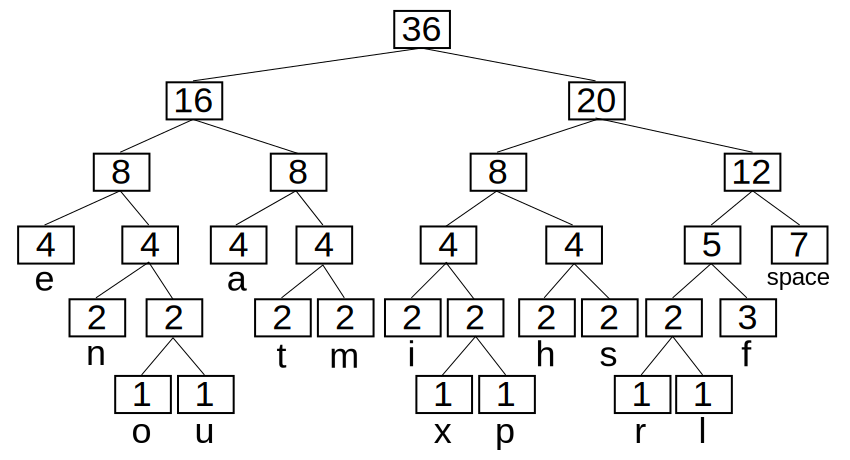
\includegraphics[scale=0.5]{figs/related_work/huffman.pdf}
    \caption{Visualisation of an example Huffman tree, created with the string "this is an example of a huffman tree" as input. Source: \citet{Dcoetzee2007}}
    \label{fig:huffman}
\end{figure}
%https://commons.wikimedia.org/wiki/File:Huffman_tree.svg

\begin{table}[h!]
\begin{tabular}{|lll||lll||lll|}
\hline
\textbf{Char} & \textbf{Freq} & \textbf{Code} & \textbf{Char} & \textbf{Freq} & \textbf{Code} & \textbf{Char} & \textbf{Freq} & \textbf{Code} \\ \hline
space         & 7             & 111           & m             & 2             & 0111          & p             & 1             & 10011         \\
a             & 4             & 010           & n             & 2             & 0010          & r             & 1             & 11000         \\
e             & 4             & 000           & s             & 2             & 1011          & u             & 1             & 00111         \\
f             & 3             & 1101          & t             & 2             & 0110          & x             & 1             & 10010         \\
h             & 2             & 1010          & l             & 1             & 11001         &               &               &               \\
i             & 2             & 1000          & o             & 1             & 00110         &               &               &               \\ \hline
\end{tabular}
\caption{Table that accompanies Figure~\ref{fig:huffman}. It contains all characters of the original string with their frequencies and the binary code with which they are mapped. Source: \citet{Dcoetzee2007}}
\label{tab:huff}
\end{table}


% Add something about performance, decoding and how strings are actually coded

\subsection{DEFLATE and zlib}
\label{sec:zlib}
Zlib is a free general purpose compression library that uses the Deflate method, which in turn is based on Huffman coding and \ac{lz77} compression.
The input data is split into a series of blocks.
Each block is compressed separately by using \ac{lz77}.
Subsequently, Huffman coding is used on the encoded blocks.
For the latter part, zlib has two different implementations that are performed on individual blocks: either with creation Huffman trees with the algorithm which is then stored alongside the data, or by using default trees that are defined in DEFLATE which removes the need of storing the extra information \citep{zlib}.

\subsection{Smaz}
\label{sec:smaz}
Even though it can be used on any kind of natural language text, Smaz is a compression library for the specific purpose of working well on small strings.
General purpose compression techniques tend to have a larger overhead in order to be able to work well with dynamic input, which is why Smaz is potentially more suitable for this specific case \citep{antirez}.
It works with a static codebook containing frequent-occurring English (fragments of) words and bigrams. 
This makes it likely to work best on English strings, however, this is subject to testing.
The parts are encoded in binary, with the most frequent parts being in the smallest representation \citep{antirez2}.
Its general idea is thus similar to Huffman coding (see \ref{sec:huffman}).

%\subsection{tar + gzip}
%This is used by Cesium (or at least in their tests), could be worth investigating.


\section{Compression of geometries, meshes, and graphs}
\subsection{Quantisation}
\label{theoryquantisation}

Quantisation is a technique that can be regarded as lossy compression.
It is used for signal processing, converting continuous data from an analogue source to a digital representation.
But it can also be applied to data that is already digitalised, for instance a list of coordinates as is exemplified by Draco in this thesis.
It works by mapping a dictionary containing all values that the data encompasses to a dictionary reduced in size, to which original values are joined many-to-one.
This means for example that a value that occurs once will be mapped to a value that is close to it but occurs more frequently, losing some of the original information \citep{sayood2017introduction}.
Vector quantisation can be used to compress coordinates \citep{rossignac20013d}.


\subsection{Delta encoding}
Another used name for this concept is delta compression.
It is for instance used for version control, the distribution of software patches, and other transmission of data over the web.
The idea behind it is to only store or transmit the delta (difference) of the data to data that is already stored or received.
The complete data can subsequently be reconstructed by adding the delta to the existing data that it is connected to \citep{suel2019delta}.
The technique can be applied within a complete set of data as well as is is for example done in \citet{deering1995geometry}, where vertices are stored in an array as a vector of the delta difference with the previous vertex.
Both transmitting deltas and storing deltas in a complete dataset are relevant for this thesis in the context of streaming and the compression of geometry as well as feature attributes.




\subsection{Edgebreaker}
\label{sec:theoryedgebreaker}

Edgebreaker is one of the techniques used by Draco to compress 3D triangle meshes.
A mesh that consists of triangles can be represented by the vertex data, which is made up of the coordinates of all vertices that the mesh encompasses, and the connectivity, which defines the relation between the triangles (or faces) and the vertices that belong to it.
This is how Wavefront OBJ files are structured as well, which is followed by CityJSON.
The Edgebreaker algorithm compresses the connectivity data of meshes \citep{rossignac2003edgebreaker}.\\

%This upper-bound on storage does not rely on statistic-based entropy or arithmetic coding schemes, which in general perform poorly on small or irregular meshes. Consequently, Edgebreaker is particularly attractive for compressing large catalogs of small models.
% van edgebreaker on a corner

\subsubsection{Compression}
To encode this information, first a spiraling triangle spanning tree is created for the mesh \citep{rossignac2003edgebreaker}. Analogised with peeling an orange, it is done by cutting around the peel in a spiraling way, after which it can be laid out flat.
This is visualised in Figure~\ref{fig:spanningtree}.
With a mesh this would result into a curled string of triangles.
Ultimately, the dual graph of this string represents the spanning tree \citep{taubin1998geometry}.\\

\begin{figure}[h]
    \centering
    \includegraphics[scale=0.8]{figs/related_work/spanningtree.jpg}
    \caption{Visualisation of the creation of a triangle spanning tree, not showing the dual graph representation. Figure taken from \citet{taubin1998geometry}}
    \label{fig:spanningtree}
\end{figure}

% https://www.sciencedirect.com/topics/computer-science/spanning-tree
% en corner-table paper
Consequently, the algorithm traverses the triangles of the spanning tree, keeping track of all visited triangles and the vertices they are bounded by.
Each triangle is assigned one character of the set \texttt{\{C,L,E,R,S\}}, which denotes one of the five cases (see Figure~\ref{fig:clers}) that are defined in the specification of the algorithm.
C means that the shared vertex v, between the current triangle and the ones to its left and right, has not been visited at all.
As for the other four cases, vertex v has been visited and the triangle left or right (L or R), both of them (E) or neither of them (S) has been traversed \citep{rossignac2003edgebreaker, rossignac20013d}.


\begin{figure}[h!]
    \centering
    \includegraphics[scale=0.8]{figs/related_work/clers.png}
    \caption{The five cases defined for the Edgebreaker method. X is the current triangle in the iteration, v the vertex that is shared between X and the triangles to its left and right, and blue triangles are unvisited. Figure taken from \citet{rossignac2003edgebreaker}}
    \label{fig:clers}
\end{figure}

During the traversion of the triangles two tables (M and U) are created to respectively store the visited vertices and triangles, and two others (V and O) are used to keep references to vertices and their opposite corners.

Optionally, a prediction method for \texttt{CLERS} symbols of succeeding unencoded triangles can be used, which is based on the vertex valences \citep{dracopredictive}.
The valency (or degree) of a vertex is the amount of edges that is emanating from it.
The addition of this method can decrease the file size in similar fashion to parallelogram prediction (see Section~\ref{sec:parallelogram}), as symbols would not have to be stored explicitly.

%https://github.com/google/draco/blob/master/src/draco/compression/mesh/mesh_edgebreaker_traversal_predictive_encoder.h
%// Encoder that tries to predict the edgebreaker traversal symbols based on the
%// vertex valences of the unencoded portion of the mesh. The current prediction
%// scheme assumes that each vertex has valence 6 which can be used to predict
%// the symbol preceding the one that is currently encoded. Predictions are
%// encoded using an arithmetic coding which can lead to less than 1 bit per
%// triangle encoding for highly regular meshes.

\subsubsection{Decompression}
Decompressing the mesh the V (vertice references) and O (opposite corners references) tables will be reconstituted, and after that the table containing the vertex positions.
The \texttt{CLERS} string is iteratively decoded to create a triangulated polygon that approaches C in Figure~\ref{fig:spanningtree}, adding one triangle at a time. 
An S triangle will invoke the start of the decompression of one string of triangles (as there are multiple ones because of recursive compression).
Encountering an E means that the end of the string is reached in the current recursion iteration.
Depending on the other symbols that are encountered, the bounding edges shown in C in Figure~\ref{fig:spanningtree} are zipped up by matching pairs of edges.
In this way, ultimately shape A in Figure~\ref{fig:spanningtree} is reconstituted.
After the decompression of the connectivity information, the positions of the vertices are decompressed \citep{rossignac2003edgebreaker}.
%An S triangle will invoke the start of the decompression of one string of triangles (as there are multiple ones because of recursive compression).
%If a C is encoutered, this means that no adjacent triangles have been decoded yet, as according to the CLERS string they were not visited at that point. 
%Therefore, no zipping of edges takes place yet.
%Only when an L is encountered, meaning that its left triangle has been visited, will a zip take place between the left edge of L and the adjacent edge of the previously visited C triangle.
%As for an R triangle, its opposite edge is labeled with -2, but no zipping is attempted. That edge is zipped later in another recursion iteration.
%Encountering an E means that the end of the string is reached in the current recursion iteration.
%This means that all free edges can be zipped, as long as the one on the right is marked with -2 and the one on the left with -1.
%It is then when R triangles are zipped as well.



%For this purpose a so-called Corner-Table, consisting of two arrays of integers, is created which describes the connectivity information.



% edgebreaker vs andere oudere algoritmes? was een paper over



\subsection{Sequential connectivity compression}
\label{sec:seqconnectivity}

An alternative method to edgebreaker that Draco can use is their own sequential connectivity method.
It either uses delta encoding (storing the difference of vertex coordinates to the ones of the previous vertex \citep{deering1995geometry} to store the IDs of vertices after which they are compressed by entropy encoding (of which Huffman coding is an example---~\ref{sec:huffman}), or the IDs are simply stored using everytime the amount of bits that the largest vertex id takes up \citep{Google2019}.
In contrast with edgebreaker, this method preserves the vertex order within triangles.
% (does it also preserve face order?) i could test myself
On the other hand the resulting encoding will not be as small.

%https://github.com/google/draco/issues/132
%It also does not use "some of the more advanced algorithms for point attribute compression (such as parallelogram prediction, etc..). This may change in future if there is demand for it.".

\subsection{Parallelogram prediction}
\label{sec:parallelogram}
Parallelogram prediction compresses meshes by predicting the missing vertex of a triangle, knowing the two vertices from the edge shared with a previously decoded triangle \citep{gotsman-touma-gi98, Google2018}.
A basic prediction can be made with the so-called parallelogram rule, as defined by formula~\ref{eq:parallelogram}, with the variables referring to the vertices in Figure~\ref{fig:parallelogram}.

\begin{equation}
r^p = v + w - u
\label{eq:parallelogram}
\end{equation}

However, this prediction can be improved by taking an estimated crease angle between the two triangles (the "crease" being the shared edge---the angles are depicted on Figure~\ref{fig:parallelogram} with the lines crossing edges (\(s,v\)) and (\(v,u\))) into account, as opposed to assuming that they are co-planar.
This angle is estimated based on at least one set of adjacent triangles, that thus has to be decoded already.
If there are more adjacent triangles available, it is taken as the average of the crease angles between the two sets of triangles that are closest to parallel to the shared edge of the current triangle and the predicted one \citep{gotsman-touma-gi98}.
As example, \(r_ca^p \) on Figure~\ref{fig:parallelogram} is the predicted vertex of the next triangle by taking the crease angles between triangles (\(s,v,t\)) and (\(s,v,w\)).

Ultimately, the mesh is compressed by storing the error of the predicted vertex to the actual vertex (as a vector) rather than the vertex itself. 
It is therefore a completely lossless technique.

\begin{figure}[h!]
    \centering
    \includegraphics[scale=0.8]{figs/related_work/parallelogram_rule.jpg}
    \caption{Illustrated how a new vertex can be predicted using parallelogram prediction. \(r^p\) is the vertex as predicted with the parallelogram rule, \(r_ca^p \) is as predicted with the crease angle taken into account. Figure adapted from \citet{gotsman-touma-gi98}}
    \label{fig:parallelogram}
\end{figure}




%\subsection{Entropy encoding}
%Huffman is one of the most common forms of entropy encoding (according to wikipedia at least).
%\citep{mackay2003information}


%\subsection{Sequential connectivity}
%This is the second method that Draco can use, but of which I could not find proper information yet.

%\subsection{Streaming meshes}
%The algorithm from the Isenburg paper.